\section{Method}
\label{sec:method}

\subsection{Tool-Existence Hallucination Rate (TEHR)}
\label{sec:method:tehr}

Let a tool registry $\mathcal{R}$ be a finite set of tool names with JSON schemas, exposed to the agent at episode start. The agent's message stream is parsed into a sequence of tool calls $c$, each carrying a name $c.\mathrm{name}$, and we define
\[
\mathrm{TEHR}(m, b, x) = \frac{|\{c : c.\mathrm{name}\notin \mathcal{R}\}|}{|\{c : c \text{ is a parsed tool call}\}|},
\]
where $m, b, x$ index model, benchmark, and condition. The denominator is per call, not per task. Per-task aggregation conflates the rate with trace length: on long tool-using episodes, a single bad agent emitting twenty bad calls swings the headline number by an order of magnitude relative to one. Per-call observations inside a task are not assumed i.i.d.; task-level cluster-bootstrap confidence intervals are reported instead. System failures (timeout, refusal, parse-fail) are excluded from numerator and denominator alike.

\subsection{Registry-Visible Reprompting (RVR)}
\label{sec:method:rvr}

\begin{figure*}[t]
\centering
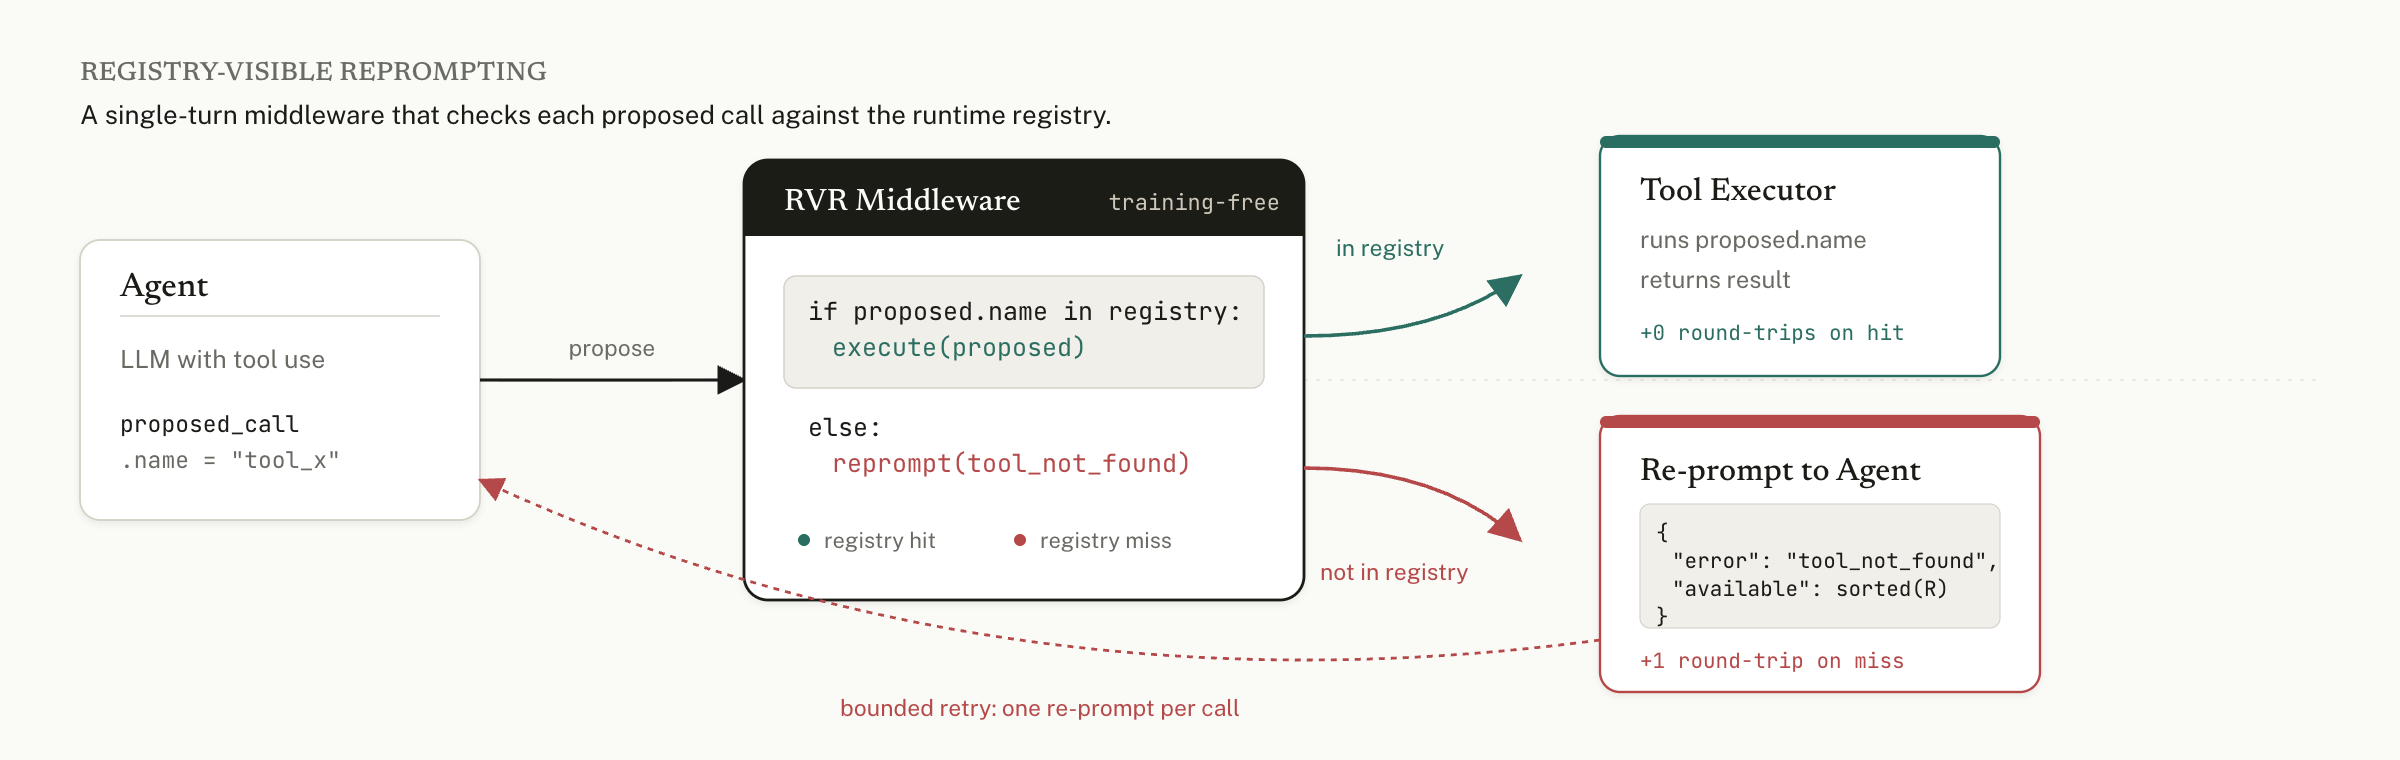
\includegraphics[width=0.85\linewidth]{figures/fig3_rvr_architecture}
\caption{RVR middleware. An $O(1)$ membership check runs in-process
on each proposed call. Hits execute. Misses trigger one re-prompt
with a structured \texttt{tool\_not\_found} envelope (and the sorted
registry under $\mathrm{C}_1$). The no-violation path adds zero
provider round-trips; the violation path adds one, bounded to a
single retry.}
\label{fig:rvr-arch}
\end{figure*}

RVR is a single-turn intervention placed between the agent and the tool executor (Figure~\ref{fig:rvr-arch}). On a membership-violating call, it returns a re-prompt that names the offending call and lists the available tools:

\begin{lstlisting}[language=Python,basicstyle=\ttfamily\footnotesize]
def rvr(agent_msg, registry):
    proposed = parse_tool_call(agent_msg)
    if proposed.name not in registry:
        return Action.RE_PROMPT(
            f"Tool '{proposed.name}' not in registry. "
            f"Available: {sorted(registry.keys())}.")
    return Action.EXECUTE(proposed)
\end{lstlisting}

Echoing $\mathcal{R}$ back into the conversation places valid names in the model's recent context, which is what the next decoding step attends to. The intervention uses one re-prompt, a production-realistic budget; it is training-free and assumes no gradient access; it composes with RL-based methods such as Fission-GRPO~\citep{fissiongrpo2026}; and it is the message-level analog of constrained decoding for closed-API regimes without logit access.

\subsection{Conditions and pre-registered mechanism hypotheses}
\label{sec:method:conditions}

Four conditions are run on a hallucinated call. \textbf{$\mathrm{C}_0$} is the opaque baseline, returning the framework's default error string. \textbf{$\mathrm{C}_{0.5}$} is a naive retry with the literal text ``previous call failed, try again''. \textbf{$\mathrm{C}_{0.7}$} is a structured error, JSON \texttt{\{"error":"tool\_not\_found"\}}, without the registry attached. \textbf{$\mathrm{C}_1$} is RVR proper (Section~\ref{sec:method:rvr}). The active comparator $\mathrm{C}_1\!:\!\mathrm{C}_{0.7}$ isolates the registry list; the secondary $\mathrm{C}_1\!:\!\mathrm{C}_{0.5}$ ablates content. At scale we report $\mathrm{C}_1\!:\!\mathrm{C}_0$, the more conservative comparator. The $\mathrm{C}_{0.5}/\mathrm{C}_{0.7}$ runs were deferred in favor of breadth (Appendix~A).

Three candidate mechanisms are pre-registered for any RVR effect. \textbf{M-Retrieve} attributes the gain to induction-head copying and predicts a near\_name peak. \textbf{M-Constrain} attributes it to message-level rejection sampling and predicts no distractor-type modulation. \textbf{M-Metacog} attributes it to a registry-as-cue effect and predicts a semantic/synonym peak. The falsifier is asymmetric: support for M-Constrain requires both Friedman non-significance \emph{and} post-hoc power $\geq 0.80$ for a $5$~pp pairwise difference. A null result alone is insufficient.

\subsection{Distractor-Type Probe}
\label{sec:method:probe}

\begin{figure}[t]
\centering
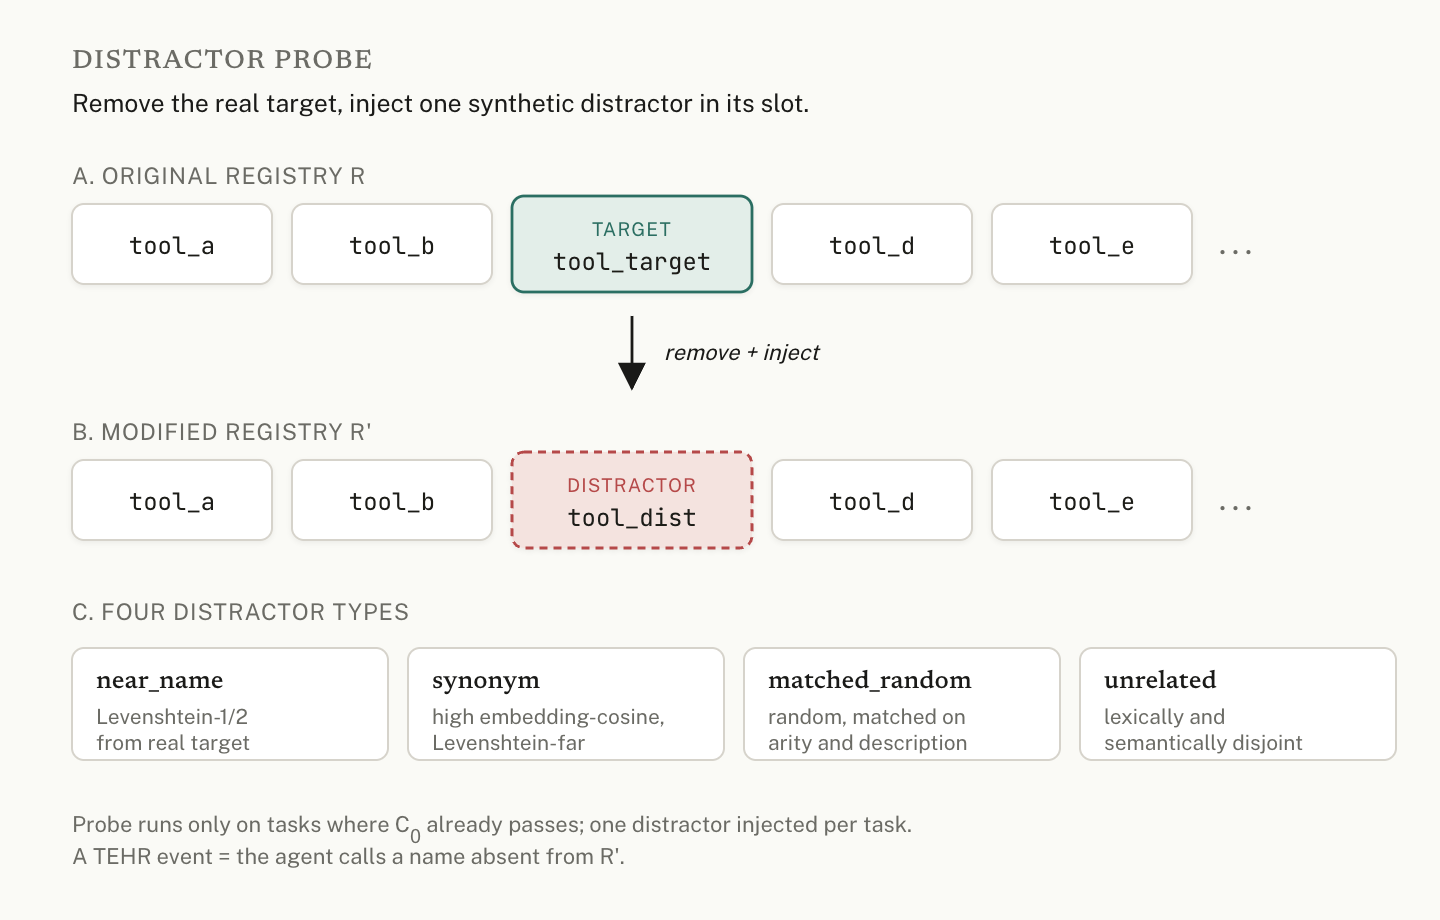
\includegraphics[width=\linewidth]{figures/fig4_distractor_probe}
\caption{The distractor probe. Starting from a registry where the
opaque baseline already passes, the real target tool is removed and
one synthetic distractor is injected in its slot. The four arms vary
the similarity profile of the distractor.}
\label{fig:probe}
\end{figure}

One distractor is injected into $\mathcal{R}$ on tasks where $\mathrm{C}_0$ already passes, with its type varied to separate the three mechanism hypotheses. \textbf{near\_name} draws a string at Levenshtein distance 1 or 2 from a real target. \textbf{synonym} is high embedding-cosine but Levenshtein-far: semantic but not orthographic overlap. \textbf{matched\_random} is lexically random, matched to the real target on description length and arity, controlling for the ``registry-size $+1$'' confound. \textbf{unrelated} is lexically and semantically disjoint, the floor case. To capture the Czapla-style runtime collision, the real target is also removed and the distractor placed in its slot: the agent expects a tool that exists, but the registry offers only a similarly-named substitute. Distractor-type differences are tested with the Friedman omnibus and Nemenyi-corrected pairwise contrasts.
